%----------------------------------------------------------------------------------------
%	PACKAGES AND OTHER DOCUMENT CONFIGURATIONS
%----------------------------------------------------------------------------------------

\documentclass{article} % Paper and 12pt font size
\usepackage[utf8]{inputenc}
\usepackage{lmodern} % Use font Latin Modern Sans Typewriter
\usepackage[a4paper, margin=1in]{geometry} % Paper size and margin
\usepackage{hyperref} % Hyperlinks

\usepackage{enumitem} % Format the enumerated list
\usepackage{amsmath,amsfonts,amsthm,mathtools} % Math packages
\setlength\parindent{0pt} % Removes all indentation from paragraphs - comment this line for an assignment with lots of text

\usepackage{array}
\usepackage{tabu} % Table to text width
\renewcommand{\arraystretch}{0.6} % If the value is 1.0, the height of each row in the table is set to 1.5 relative to its default height. Adjust based on that.
\usepackage[table]{xcolor}

\usepackage{tikz} % Remember picture
\usepackage{graphicx} % Includes images
\graphicspath{ {./images/} } % Tells LATEX that the images are kept in a folder named images under the directory of the main document
\usepackage{subcaption}
\usepackage{caption}
\usepackage{wrapfig} % Wrap image i
\usepackage{eso-pic} % used for image background on titlepage

% Code listing style --------------
\usepackage{listings} % Code listing
\usepackage{color}
\definecolor{codegreen}{rgb}{0,0.6,0}
\definecolor{codegray}{rgb}{0.5,0.5,0.5}
\definecolor{codepurple}{rgb}{0.58,0,0.82}
\definecolor{backcolour}{rgb}{0.95,0.95,0.92}
\lstdefinestyle{mystyle}{
    backgroundcolor=\color{backcolour},
    commentstyle=\color{codegreen},
    basicstyle=\ttfamily\small,
    keywordstyle=\color{magenta},
    numberstyle=\tiny\color{codegray},
    stringstyle=\color{codepurple},
    breakatwhitespace=false,
    breaklines=true,
    captionpos=b,
    keepspaces=true,
    numbers=left,
    numbersep=5pt,
    showspaces=false,
    showstringspaces=false,
    showtabs=false,
    tabsize=2
}
\lstset{style=mystyle}

%----------------------------------------------------------------------------------------
%	TITLE SECTION
%----------------------------------------------------------------------------------------
\title{\Huge \textbf{Bayesian Logistic Regression} \vspace{.4in} \hrule}

\author{%\LARGE University of Toronto Institute for Aerospace Studies\\
  \vspace{0.5cm}
	\Large ROB313: Introduction to Learning from Data \\
  \vspace{0.5cm}
	\Large Yizhi (Jojo) Zhou, 1003002396\\
}
\date{\normalsize\today}

\linespread{1.5}

\begin{document}
	\begin{titlepage}
	\tikz[remember picture,overlay]
	\node[yshift=8.0cm] at (current page.south){
\includegraphics[width=\paperwidth]{BG.png}};%height=\paperheight and (current page.south)
	\vspace*{3.5cm}
  {\let\newpage\relax\maketitle}
	\vspace*{\fill}

	\end{titlepage}

\newpage

%----------------------------------------------------------------------------------------
%	PROBLEM 1
%----------------------------------------------------------------------------------------
\vspace{0.3cm}
\section*{Objectives} % The * makes it an unnumbered section
In this project, Bayesian logistic regression is used to predict the binary results of one class in the Iris dataset, with a Bernoulli likelihood. The following report briefly describes the implementation of the different appriximation methods that improves the efficiency of Bayesian logistic regression, studies the influence on different parameters/models proposed before the training, as well as the performance of Bayesian compared to the frequentist approach. The report is then ended by a brief report on a summary paper from P. Domigos.


%----------------------------------------------------------------------------------------
%	PROBLEM 1
%----------------------------------------------------------------------------------------
\vspace{0.3cm}
\section*{Solution Structure and Strategies} % The * makes it an unnumbered section
The implemention is composed of the following 4 parts, with more details in the Jupyter Notebook\footnote{The Jupyter Notebook is attached in the submitted folder.}:
\begin{itemize}
  \item \textbf{Probability Functions}
    This section includes all the log of likelihood P(y|$w$, x), prior distribution P($w$), and the log of posterior distribution which is the sum of these two, as well as their gradients and hessians which will all be later used, for example, when finding the Maximum A Posterior of w, and when calculating the importance weights of each sample of $w$.
    \begin{minipage}{\linewidth}
      \raggedright
      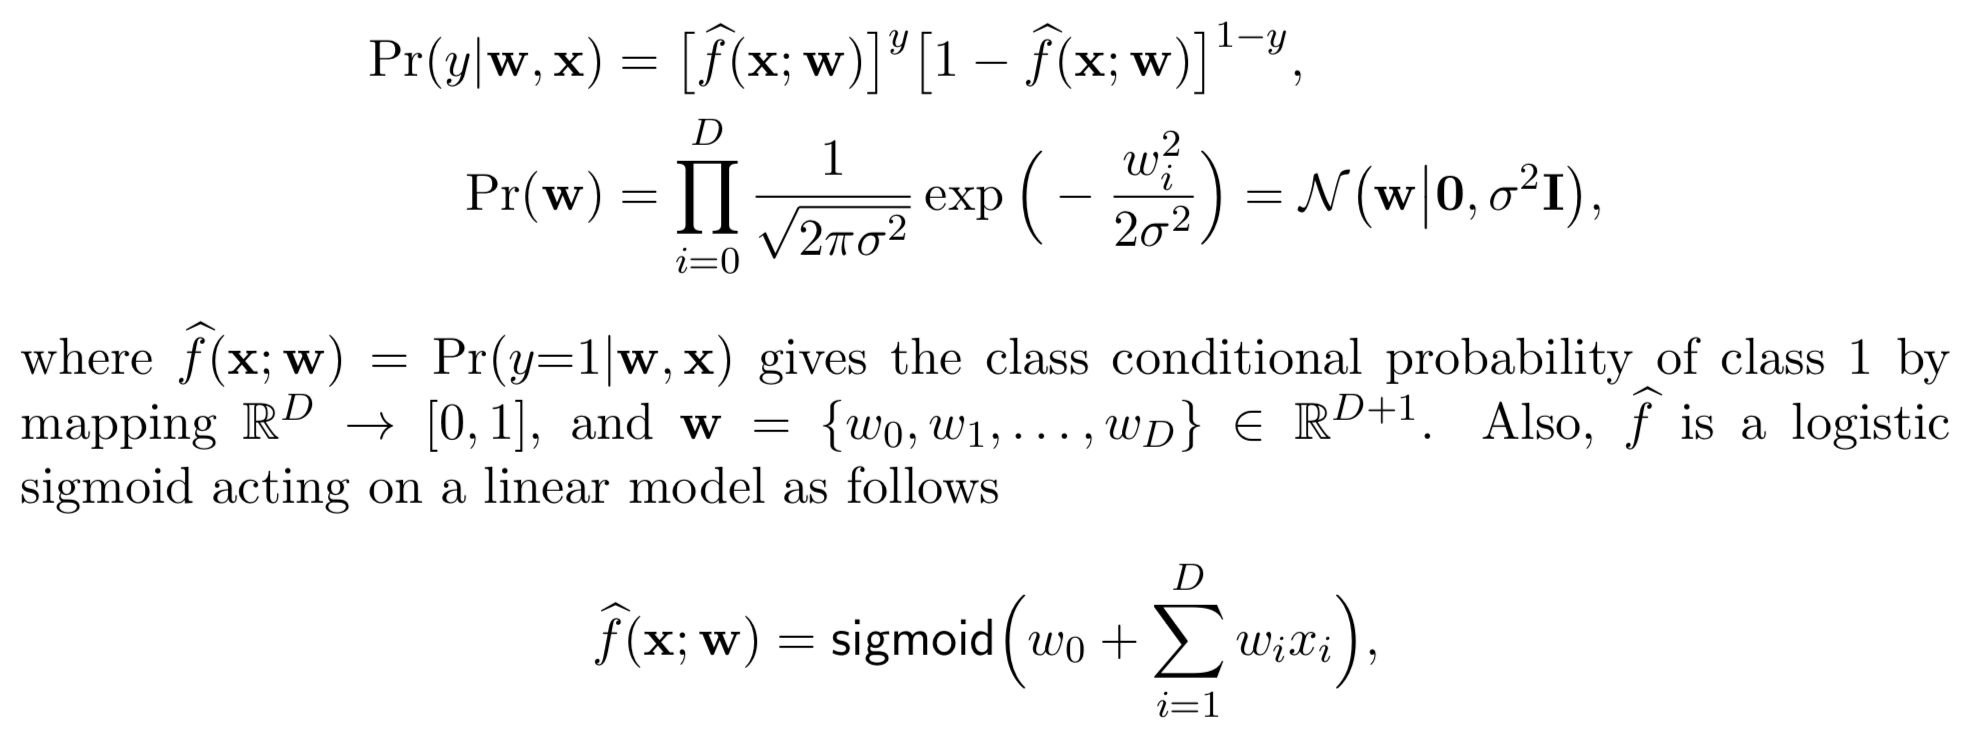
\includegraphics[width=\textwidth]{Equations.png}
    \end{minipage}

  \item \textbf{Bayesian with Laplace Approximation}
  \begin{itemize}
    \item \textit{Gradient Ascent.} The Maximum A Posterior ($w_{MAP}$) is obtained by performing a Gradient Ascent to maximize the log of posterior probablity. It has an iteration cap and is early-stopped as soon as the gradient's largest value is smaller than the errorbound.

    \item \textit{Bayesian Logistic Regression.} This is the main body of Question 1, implemented in a class. It initialzes the prior distribution with different $\sigma^2$ values and computes the $w_{MAP}$ corresponding to that distribution. The models with different $\sigma^2$'s are then compared by their marginal likelihood. The results are shown in the next section.
  \end{itemize}

  \item \textbf{Importance Sampling}
  Question 2 is implemented in one class, using the probability functions from before. Instead of computinbg one ``optimal'' $w$, however, this model directly uses predictions generated from all the $w$'s drawn from the proposal distribution, weighted by their importance (proportional to the likelihood, prior, and inversely proportional to the proposal, at each $w$). The accuracy of prediction, as well as the sampling process is visualized and discussed.

  \item \textbf{Metropolis-Hastings MCMC Sampling}
  This class follows the same structure with the previous one, except for its different method of sampling. Instead of randomly generating a number of samples from the proposal distribution, it tries one random step each time from the proposal distribution, but rejests it if criteria are not met. After 1000 burn-in steps, the algorithm then takes 1 sample in every 100 steps, using which to perform the prediction as in Importance Sampling.
\end{itemize}



%----------------------------------------------------------------------------------------
%	PROBLEM 2
%----------------------------------------------------------------------------------------
\vspace{0.3cm}
\section*{Bayesian Logistic Regression} % The * makes it an unnumbered section

{\large\textbf{Bayesian likelihoods with different variances of the prior distribution}}

  With each prior distribution having a variance of $\sigma^2 =$ 0.5, 1, or 2, respectively, the marginal likelihood of its posterior distribution which is approximated by the Laplace model, is presented in Figure 1.

  \begin{wrapfigure}{r}{0.7\textwidth}
    \begin{center}
      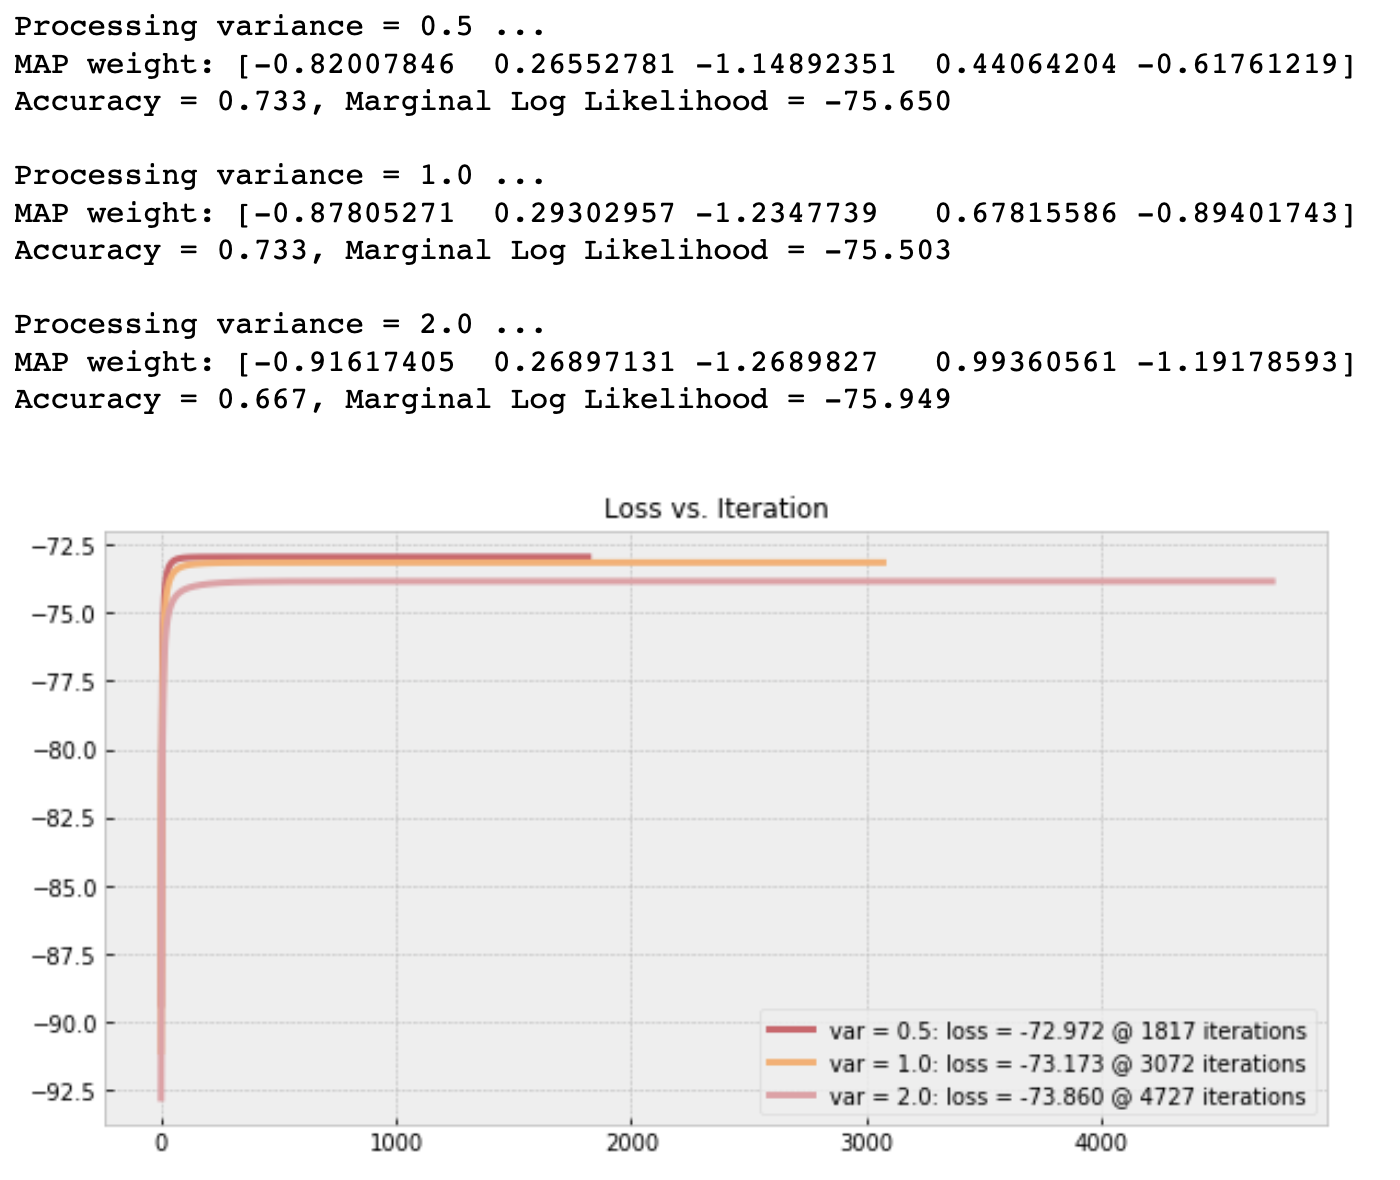
\includegraphics[width=0.6\textwidth]{A5_1.png}
    \end{center}
    \caption{Upper: Results from Laplace approximation. \\Lower: Gradient Ascent in finding $w_{MAP}$}
  \end{wrapfigure}

  As can be seen from the marginal likelihoods, the model's performance isn't in a linear relationship with the variance; instead, it decreases when the variance goes up to 1 and increases again when the variance keeps going to 2. This reflects the concept of \textbf{bias-variance tradeoff}, where model complexity increases with the variance where the model is considered ``overfitted'', and decreases with bias where it is ``underfitted''. The goal is to find a sweet spot in between underfitting and overfitting, where neither the variance or bias is minimized but the model performance is optimized. In this case, the model with $\sigma^2 =$2 is the most complex, also reflected from the fact that it took the most iterations (under the same other parameters such as learning rate) to reach to the $w_{MAP}$. Meanwhile, \textbf{$\sigma^2 =$ 1 returns the best result amoung all}, indicating that it is closer to the optimal model complexity regarding the bias-variance tradeoff; as a result, its accuracy on the test set is also higher than the overfitted model with $\sigma^2 =$2.

    \begin{figure}[!hbt]
      \centering
      \begin{subfigure}[b]{0.85\linewidth}
        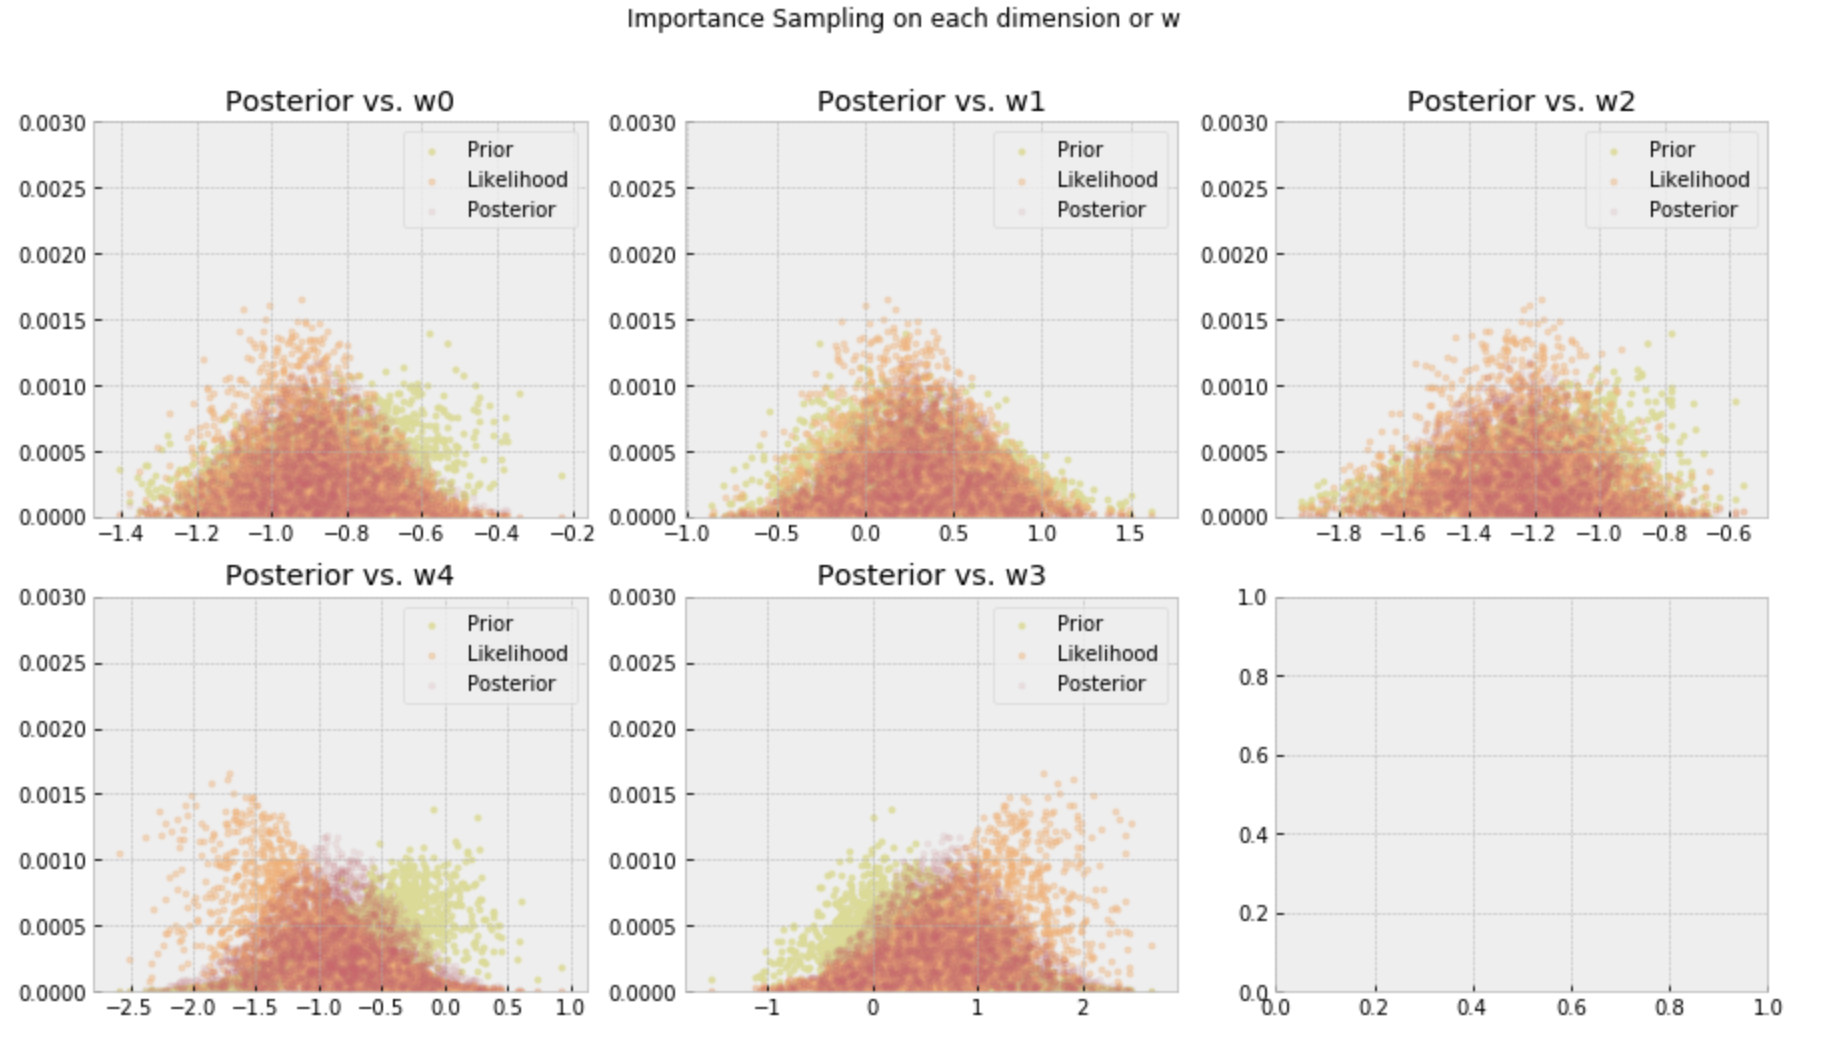
\includegraphics[width=\linewidth]{A5_2_1.png}
        \caption{Laplace appriximation with $\sigma^2=1$}
      \end{subfigure}
      \begin{subfigure}[b]{0.85\linewidth}
        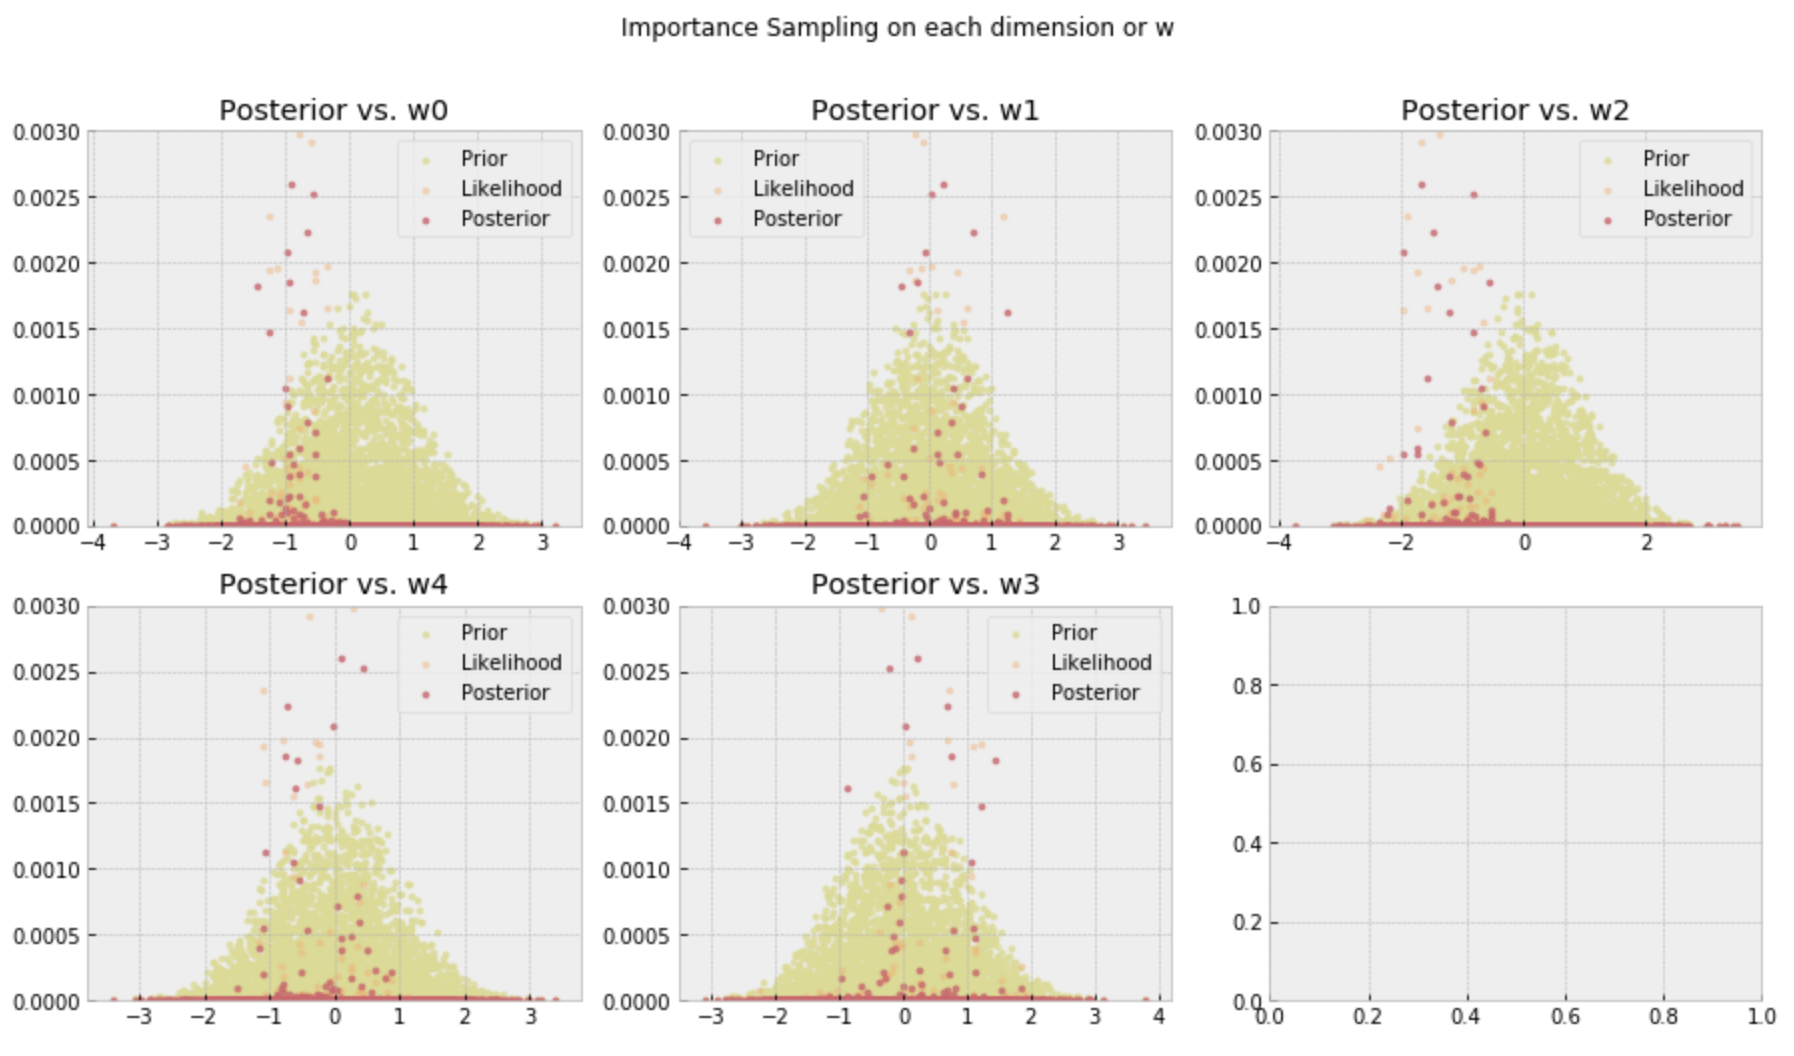
\includegraphics[width=\linewidth]{A5_2_2.png}
        \caption{Direct Gaussian with $\mu=0, \sigma^2=1$}
      \end{subfigure}
      \caption{Visiualization of posterior, prior, and likelihood, with different proposal distributions}
      \label{fig:Q1_1}
    \end{figure}

\vspace{1cm}
{\large\textbf{Importance sampling and its performance}}

  In face, as long as the proposal distribution isn't too far away from the actual underlying one, the prediction always converge with a large enough amount of samples chosen, as the importance weights eventually correct the bias introduced by sampling from the wrong distribution. The difference is in the amount needed, which is significantly larger for bad proposals and small for good ones. In this case, \textbf{the Laplace model computed with a prior distribution of $\sigma^2 =$ 1 is chosen as the proposal distribution}, since it is the closest to the actual underlying distribution without extra computation. Figure 2 shows the visualization on each dimension with the chosen proposal distribution, as well as a dummy proposal of simply a zero-mean Gaussian model with variance of 1. It is clear that the samples drawn are completely different, while the accuracies are essentially the same, both being 73.3\% on the test set with 3000 samples. It has been tested and shown that, however, when only 3 samles are chosen, the Laplace approximation as the proposal leads to a 66.7\% accuracy while the dummy one led to a 46.7\%, which agrees with the expectation.


\vspace{1cm}
{\large\textbf{Metropolis-Hastings MCMC sampler and its performance}}

  The implementation of MCMC sampler is already discussed in the second section of the report. The variance doesn't actually contribute to the performance of prediction - whatever the varience is set to be, the prediction accuracy is 73.3\% over the test set. The difference that it makes is the rejection rate -- in this case, $\sigma^2_p = 1$ leads to a rejection rate of about 90\%, while $\sigma^2_p = 0.05$ leads to that of about 65\%, showing the relationship that \textbf{a smaller variance leads to a lower, more desirable rejection rate}.

  With the chosen $\sigma^2_p = 0.05$, Figure 3 shows the  predictive posterior class-conditional probability samples for the 9th, and the 10th datapoints in the test set as histograms. Though both datapoints are correctly predicted to be ``False'', it is obvious that the 9th one is way more certain to be ``False'' (i.e. the probabilities of being ``True'' have an average close to 0 and a very small variance), while the 10th one is a lot less certain (i.e. the average probability is close to 0.5 and has a large variance). If it were a frequentist approach, which only cares about the most likely paramater rather than a whole list of 100 samples, it could still result in a similar prediction (in terms of accuracy) as well as its confidence indicates in how close the sigmoid value is to 0.5, but it couldn't ever show the distribution of predictions resulting from different parameters - it would never know how the performance/results would change with even small changes of that optimized parameter. For example, the 9th datapoint in this case has featured that would lead to a similar, correct prediction under slight changes of the parameter, while the 10th datapoint varies a lot under such changes. As frequentist approaches essentially doesn't deal with the variance in the uncertainty, they loses such idea of confidence level and are therefore prone to misinterpretations of the values.

  \begin{figure}[!h]
    \centering
    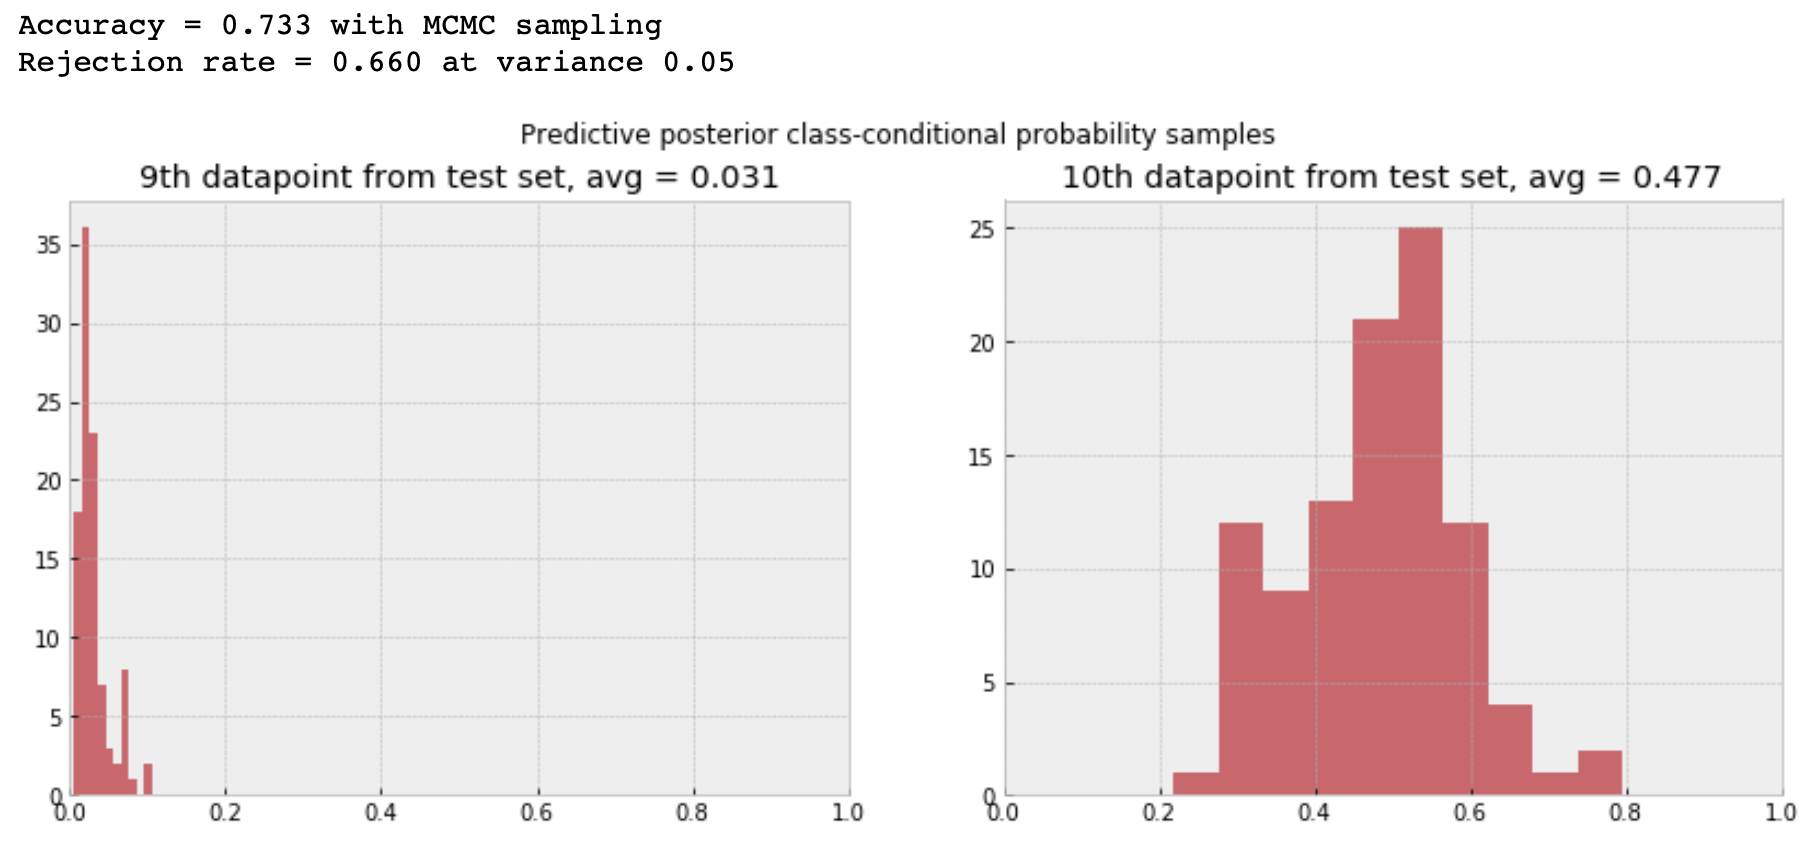
\includegraphics[width=0.85\linewidth]{A5_3.png}
    \caption{Distribution of predictions on two datapoints}
    \label{fig:4}
  \end{figure}


%----------------------------------------------------------------------------------------
%	PROBLEM 4
%----------------------------------------------------------------------------------------
\vspace{0.3cm}
\section*{Brief Literature Review} % The * makes it an unnumbered section
{\large\textbf{Paper Source}}

  Domingos, P. \textit{A few useful things to know about machine learning}. Communications of the ACM, 55(10), pp. 78–87, 2017. \url{https://homes.cs.washington.edu/~pedrod/papers/cacm12.pdf}

\vspace{1cm}
{\large\textbf{Thoughts}}

  The paper summarizes some ``folk wisdom'' of machine learning, which, for a beginner like myself, is a great way to have some pitfalls and priorities in mind for my future studies and practices. Some of the topics already resonate with my experiences from the previous assignments in this course. For example, the warning that the training set and test set must never be mixed is also reflected in the Mauna\_Loa dataset, where the range of test set's features are disjoint from that of the train set; as a result, when using the train set itself to see the performance, it falsely gives a high accuracy opposite to what the test set generates, especially when using nonparametric methods like kNN. This dataset has also verified the importance of feature engineering, the 7th point in the article.
  When using the Generalized Linear Model as a representation, the basis functions is the key to successful fitting; the sinusoidal mapping of features gave a high accuracy while a Gaussian fitting was dreadful.


  The representation models and optimization techniques we've learned so far are limited, so some other parts of this article are yet to be experienced and then understood. For example, though the Mnist Small dataset has more than 700 dimensions, the impact of high dimensionality hasn’t been obvious to us in either the time efficiency or the understanding of how different dimensions contribute to the prediction, both in terms of runtime and accuracy. I greatly appreciate the table listing the different representations, evaluations, and optimizations in the beginning of the paper - It would be great if the article could explain more about their different usages and connect them better with the rest lessons. As mentioned in the 8th point in the article, being smart of designing or choosing the features is the hardest part of machine learning and usually takes the longest time. Other than simply warning us, however, it would be even more helpful if a chart of pros and cons or studies done on each model(method) could be summarized as well.

\end{document}
